%  LaTeX support: latex@mdpi.com
%  Built on the official MDPI template, version 20260911 (see TEMPLATE_PROVENANCE.md).
%=================================================================
\documentclass[information,article,submit,moreauthors]{Definitions/mdpi}

% Numbers, tables and figures are generated from the frozen analysis artifacts
% by scripts/make_manuscript_inputs.py and scripts/make_manuscript_figures.py.
% No result below is typed as a literal.
% Generated by scripts/make_manuscript_inputs.py from frozen artifacts.
% Do not edit. Every result in the manuscript resolves through these.
\newcommand{\NumCalibrationItems}{300}
\newcommand{\NumCalibrationRecords}{4,800}
\newcommand{\NumCoordinates}{3}
\newcommand{\NumDatasets}{2}
\newcommand{\NumHeldOutItems}{600}
\newcommand{\NumHeldOutRecords}{28,800}
\newcommand{\NumModelFamilies}{2}
\newcommand{\NumModelsConditions}{4}
\newcommand{\NumSeedRecords}{18,432}
\newcommand{\NumSmokeItems}{32}
\newcommand{\NumSmokeRecords}{1,536}
\newcommand{\NumTotalRecords}{53,568}
\newcommand{\NumContrasts}{16}
\newcommand{\NumChangeDetected}{1}
\newcommand{\NumEquivalent}{1}
\newcommand{\NumInconclusive}{14}
\newcommand{\MarginRisk}{0.025}
\newcommand{\MarginCoverage}{0.05}
\newcommand{\BootstrapReplicates}{5,000}
\newcommand{\MaxRealisationEquivalent}{0.015}
\newcommand{\MinRealisationNonEquivalent}{0.115}
\newcommand{\NumAllAnswersChanged}{7}
\newcommand{\DetectedModel}{Qwen3.5-9B thinking}
\newcommand{\DetectedDataset}{ManyIFEval}
\newcommand{\DetectedShift}{high-$T$}
\newcommand{\DetectedDeltaR}{+0.016}
\newcommand{\DetectedCILow}{+0.007}
\newcommand{\DetectedCIHigh}{+0.026}
\newcommand{\DetectedHolmP}{0.003}
\newcommand{\MaxCoverageModel}{Ministral-3-8B instruct}
\newcommand{\MaxCoverageDataset}{SuperGPQA}
\newcommand{\MaxCoverageShift}{high-$T$}
\newcommand{\MaxCoverageDeltaK}{-0.357}
\newcommand{\MaxCoverageDeltaR}{+0.011}
\newcommand{\MaxAnswerFailModel}{Ministral-3-8B reasoning}
\newcommand{\MaxAnswerFailDataset}{SuperGPQA}
\newcommand{\MaxAnswerFailShift}{low-$p$}
\newcommand{\MaxAnswerFailDeltaQ}{+0.153}
\newcommand{\NumRiskTargetAttained}{1}
\newcommand{\NumRiskTargetInfeasible}{7}
\newcommand{\TargetRisk}{0.1}
\newcommand{\FixedCoverageTarget}{0.5}
\newcommand{\OvershootModel}{Ministral-3-8B instruct}
\newcommand{\OvershootDataset}{SuperGPQA}
\newcommand{\OvershootCoverage}{0.790}
\newcommand{\NumBSSBelowZero}{8}
\newcommand{\NumQualityPairs}{8}
\newcommand{\NumAurocContainsChance}{2}
\newcommand{\NumAurocAboveChance}{5}
\newcommand{\NumAurocBelowChance}{1}
\newcommand{\MinAuroc}{0.447}
\newcommand{\MaxAuroc}{0.873}
\newcommand{\MinGap}{+0.240}
\newcommand{\MaxGap}{+0.748}
\newcommand{\RankingCaseModel}{Qwen3.5-9B thinking}
\newcommand{\RankingCaseDataset}{ManyIFEval}
\newcommand{\RankingCaseAuroc}{0.873}
\newcommand{\RankingCaseBSS}{-3.894}
\newcommand{\RankingCaseMCB}{4.022}
\newcommand{\RankingCaseDSC}{0.128}
\newcommand{\RankingCaseAccuracy}{0.053}
\newcommand{\RankingCaseMeanC}{0.361}
\newcommand{\MinDistinctConfidence}{9}
\newcommand{\MaxDistinctConfidence}{21}
\newcommand{\MaxAtomMass}{0.73}
\newcommand{\NumCannotFitBand}{12}
\newcommand{\NumCanFitBand}{4}
\newcommand{\MaxWidthRatio}{3.6}
\newcommand{\MinAcceptedN}{138}
\newcommand{\MaxAcceptedN}{474}
\newcommand{\NumSeedSignFlipRisk}{8}
\newcommand{\NumSeedContrasts}{16}
\newcommand{\NumSeedSignFlipAll}{18}
\newcommand{\NumSeedEndpointCombos}{48}
\newcommand{\NumVarianceSplits}{68}
\newcommand{\NumSeedShareAboveHalf}{62}
\newcommand{\MedianSeedShare}{0.642}
\newcommand{\MinSeedShare}{0.171}
\newcommand{\MaxSeedShare}{0.783}
\newcommand{\NumSeedSDExceedsMargin}{5}
\newcommand{\MaxSeedSD}{0.116}
\newcommand{\SeedSubsetItems}{128}
\newcommand{\SeedList}{1729, 2718, 3141}
\newcommand{\NumSeeds}{3}


\usepackage{pgfplots}
\pgfplotsset{compat=1.18}

% Journal metadata required by the MDPI class. Completed by the editorial
% office on acceptance; the placeholders below are the template defaults.
\pubvolume{1}
\issuenum{1}
\articlenumber{0}
\pubyear{2026}
\copyrightyear{2026}
\datereceived{ }
\daterevised{ }
\dateaccepted{ }
\datepublished{ }

\Title{Portability of Confidence-Threshold Policies Under
Inference-Configuration Shift in Open-Weight Language Models}

\newcommand{\orcidauthorA}{0000-0002-5461-8899}
\newcommand{\orcidauthorB}{0000-0002-9680-2758}
\newcommand{\orcidauthorC}{0000-0001-5055-6347}
\newcommand{\orcidauthorD}{0000-0001-9280-1048}
\newcommand{\orcidauthorE}{0000-0002-0097-1873}

\Author{Nurgali Kadyrbek $^{1,}$*\orcidA{}, Madina Mansurova $^{1,}$*\orcidB{},
Octavian Adrian Postolache $^{2}$\orcidC{}, Aigerim Mekemtasovna Tleulesova $^{1}$\orcidD{}
and Syrym Kasenov $^{1}$\orcidE{}}

\AuthorNames{Nurgali Kadyrbek, Madina Mansurova, Octavian Adrian Postolache,
Aigerim Mekemtasovna Tleulesova and Syrym Kasenov}

\address{%
$^{1}$ \quad Faculty of Mechanics and Mathematics, Al-Farabi Kazakh National
University, Almaty, Kazakhstan; kadyrbek.nurgali@kaznu.kz (N.K.);
madina.mansurova@kaznu.edu.kz (M.M.); Aygerym.Tleulesova@kaznu.edu.kz (A.M.T.);
kassenov.syrym@kaznu.kz (S.K.)\\
$^{2}$ \quad Instituto Universit\'ario de Lisboa (ISCTE-IUL), Lisbon, Portugal;
Octavian.Adrian.Postolache@iscte-iul.pt (O.A.P.)}

\corres{Correspondence: kadyrbek.nurgali@kaznu.kz (N.K.);
madina.mansurova@kaznu.edu.kz (M.M.)}

\abstract{Language models are increasingly asked to report confidence scores.
A downstream policy may then accept an answer only when its score exceeds a
threshold. The threshold is selected under one inference configuration but may
later be used under different decoding settings. We ask whether the resulting
decision policy remains statistically reliable after such a change. We evaluate
\NumModelsConditions{} model conditions spanning \NumModelFamilies{} open-weight
families and two reasoning regimes, on \NumDatasets{} benchmarks with
structurally different success events, under \NumCoordinates{} inference
configurations defined relative to each model's native reference, with every
item evaluated under every configuration. Thresholds are frozen on a disjoint calibration split
and never revisited. At the reference configuration, all \NumQualityPairs{}
model--dataset pairs score worse as probability forecasts than a constant
base-rate forecast, while ranking ability varies widely, showing that
probability quality and ranking ability are distinct. Under shift, a Holm-adjusted change in
selective risk is detected in only \NumChangeDetected{} of \NumContrasts{}
contrasts, whereas
coverage moves by as much as \MaxCoverageDeltaK{} at nearly unchanged risk. A
precision analysis shows that for \NumCannotFitBand{} of \NumContrasts{}
contrasts the 95\% interval was wider than the whole equivalence region,
because risk is estimated only on accepted items. A \NumSeeds{}-seed robustness subset
shows risk-change signs reversing in \NumSeedSignFlipRisk{} of
\NumSeedContrasts{} contrasts. We conclude that confidence-threshold policies
should be validated under their intended inference configuration and evaluated
across sampling seeds.}

\keyword{large language models; uncertainty quantification; confidence
calibration; selective prediction; stochastic decoding; inference-time
robustness; decision support; probabilistic forecasting}

\begin{document}

\section{Introduction}

Language models built on the transformer architecture~\cite{vaswani2017} are
now deployed at a scale where their outputs are acted upon rather than merely
read. A model that reports a probability alongside its answer invites an
obvious operational use: accept the answer when the reported probability clears
a threshold, and route the rest to a human. This pattern is selective
prediction~\cite{chow1970,elyaniv2010foundations,geifman2017selective} applied
to generated text, and it is attractive because it needs no access to model
internals and no retraining. The threshold is chosen once on data where
correctness is known, usually to limit the error rate among accepted answers or
to obtain a target coverage.

Choosing that threshold requires fixing an inference configuration: a
temperature, a nucleus~\cite{holtzman2020nucleus} or top-$k$ truncation, a token
budget. Deployment does not hold those fixed. Serving stacks change defaults,
operators trade diversity against latency, a reasoning mode is switched on, and
a configuration chosen for throughput replaces the one used during validation.
The threshold, however, is a number in a configuration file, and it travels
unchanged.

This paper asks whether that is safe. We treat it as a portability question
rather than as a study of decoding parameters. Let $\theta_0$ be the
configuration under which a threshold $\tau_{\theta_0}$ was fixed, and let
$R_\theta(\tau)$ be the selective risk---the probability that an accepted answer
is wrong. The quantity of interest is the change

\begin{equation}
\Delta R_{\theta_0 \rightarrow \theta}
= R_\theta(\tau_{\theta_0}) - R_{\theta_0}(\tau_{\theta_0}),
\label{eq:estimand}
\end{equation}

\noindent
the change in selective risk when a fixed threshold is used after decoding
changes.

Two things make this harder to measure well than it first appears, and both
shape our design. First, selective risk is conditional on acceptance, so it can
stay flat while the system changes drastically: a configuration that stops
accepting most items can hold its risk constant and still deliver far less
work. Reporting $\Delta R$ alone hides that. Second, generation is stochastic,
so a single run per item yields an estimate conditional on one draw from the
decoder, and resampling items does not address that~\cite{song2025greedy}.

We therefore report an explicit outcome partition alongside the conditional
endpoint, score the reported confidence as a probability forecast using a proper
scoring rule with the CORP decomposition~\cite{brier1950,dimitriadis2021corp},
and run a secondary repeated-seed experiment to separate item-sampling
uncertainty from decoder-sampling uncertainty.

\paragraph{Contributions.}
\begin{enumerate}[leftmargin=*,labelsep=4.5mm]
\item A formal operational framework in which every evaluated item falls into
exactly one of five outcomes, so that a decoder shift's effect on a frozen
policy is decomposed into accepted-correct, accepted-wrong, answer-generation
failure, confidence-generation failure and low-confidence abstention, with
coverage and selective risk derived from them (Section~\ref{sec:framework}).
\item A paired, item-clustered evaluation of \NumContrasts{} prespecified
frozen-policy contrasts across \NumModelsConditions{} model conditions and
\NumDatasets{} benchmarks, with thresholds fixed on a disjoint split before any
held-out data were generated (Sections~\ref{sec:design}--\ref{sec:results}).
\item Evidence that reported confidence can rank errors well while being a poor
probability forecast, quantified by the CORP decomposition rather than by a mean
gap (Section~\ref{sec:refquality}).
\item A precision analysis showing that a selective-risk estimate is based only
on accepted items, which determines whether an equivalence question is
answerable at all (Section~\ref{sec:precision}).
\item A manipulation check showing that the same nominal decoder change does
not produce the same output changes across models, and a repeated-seed analysis
showing that decoder-sampling variability is frequently the larger component of
the variance in the measured effect
(Sections~\ref{sec:realisation}--\ref{sec:seeds}).
\end{enumerate}

\section{Related Work}

\subsection{Confidence and calibration in language models}

Neural classifiers are known to be miscalibrated in ways that do not follow from
their accuracy~\cite{guo2017calibration}, and post-hoc remedies operate on the
score rather than the model~\cite{zadrozny2002,niculescu2005}. For language
models the natural analogue is a verbalized confidence, elicited in the output
text. Recent work studies how to elicit it, whether it is faithful to the
model's internal state, and how to improve
it~\cite{tian2023calibration,ulmer2024calibrating,yona2024faithful,xu2024sayself}.
Uncertainty can also be estimated without asking the model, for instance from
an ensemble of predictors~\cite{lakshminarayanan2017ensembles}, but such routes
require either multiple models or access the deployment may not have. Our
concern is downstream of that literature: we take a native, coupled
elicitation as given and ask what happens to a policy built on it when inference
settings move.

\subsection{Selective prediction and abstention}

The reject option is classical~\cite{chow1970} and its modern treatment supplies
the risk--coverage vocabulary we use~\cite{elyaniv2010foundations,%
geifman2017selective}. Confidence thresholds are also used to control adaptive
computation~\cite{schuster2021consistent}. This literature generally assumes a
fixed predictor; the object of study here is what happens when the predictor's
inference configuration, rather than its weights, changes underneath a fixed
threshold.

\subsection{Stochastic decoding and evaluation variability}

Nucleus sampling~\cite{holtzman2020nucleus} and temperature are standard
controls, and their effect on task performance has been measured
directly~\cite{renze2024temperature}. Evaluation practice has been criticised
for ignoring the resulting non-determinism, with single-run results shown to be
unstable across benchmarks~\cite{song2025greedy}. We build on that observation in
a specific direction: rather than asking whether accuracy is stable, we ask
whether a decision policy established at one configuration retains its
reference selective risk at another, and we quantify how much of the measured
change is attributable to the sampling seed.

\subsection{Probabilistic forecast evaluation}

Because the elicited confidence is presented as a probability, it should be
scored by a proper scoring rule~\cite{brier1950,gneiting2007proper}, and
calibration and sharpness should be separated rather than
conflated~\cite{gneiting2007sharpness}. Murphy's decomposition of the Brier
score~\cite{murphy1973} has a modern, bin-free implementation in the CORP
framework~\cite{dimitriadis2021corp,dimitriadis2024triptych}, which uses
isotonic regression~\cite{ayer1955} in place of arbitrary binning. We adopt CORP
because it distinguishes two failures that a mean confidence--accuracy gap
cannot.

\subsection{Reliability of deployed language-model systems}

Work in this journal has examined decision support under the competing demands
of accuracy, transparency and trust~\cite{kovari2024decision}, uncertainty
quantification intended to be legible to a human
decision-maker~\cite{bhattacharjee2025entropy}, and the reliability of deployed
model-based assistants~\cite{alghamdi2024healthcare,darwish2025hallucination}.
Our contribution is narrower and complementary: a measurement of whether the
threshold policy underlying such a system remains reliable after a change in
how the model is run.

\section{Formal Framework}
\label{sec:framework}

\subsection{Items, answers and confidence}

Let $X_i$ denote a task item and $\theta$ an inference configuration. Running
the model produces an answer $A_{i\theta}$ and, in a second pass conditioned on
that answer, a reported confidence $C_{i\theta} \in [0,1]$. Task success
$Y_{i\theta} \in \{0,1\}$ is determined by the benchmark's own scorer. The item
is the experimental unit; configurations are within-item interventions.

Either generation can fail to produce a parsable result, and we treat those as
outcomes rather than as missing data. Write $V^A_{i\theta}$ for the event that
the answer parses and $V^C_{i\theta}$ for the event that the confidence parses.

\subsection{The frozen policy and its outcome partition}

A confidence policy with threshold $\tau$ accepts item $i$ when the answer
parses, the confidence parses, and the confidence clears the threshold:

\begin{equation}
\delta_\tau(i,\theta) = \mathbf{1}\!\left[V^A_{i\theta} \wedge V^C_{i\theta}
\wedge C_{i\theta} \ge \tau\right].
\label{eq:policy}
\end{equation}

\noindent
Requiring a parsable answer matters: a malformed answer carrying a usable
confidence is not an accepted error, it is a failure to produce work.

Every item then falls into exactly one of five outcomes, giving the partition

\begin{equation}
1 = S + E + q + a_C + a_\tau,
\label{eq:partition}
\end{equation}

\noindent
where $S$ is accepted-and-correct, $E$ is accepted-and-wrong, $q$ is
answer-generation failure, $a_C$ is confidence-generation failure given a valid
answer, and $a_\tau$ is abstention by a valid but low confidence. Coverage and
selective risk are derived quantities,

\begin{equation}
K = S + E, \qquad R = \frac{E}{K}, \qquad S = K(1-R).
\label{eq:derived}
\end{equation}

\noindent
Equation~\eqref{eq:partition} is what makes the conditional endpoint safe to
report. Two configurations can share a value of $R = E/(S+E)$ and differ
enormously in $K$, and therefore in how much useful autonomous work the policy
delivers. The primary estimand of Equation~\eqref{eq:estimand} is accompanied
throughout by the five components.

\subsection{Conditioning on the sampling seed}

Generation is stochastic. Writing $D(X,s)$ for an item's paired contribution to
a contrast at sampling seed $s$, the target usually of interest averages over
both items and decoder sampling:

\begin{equation}
\Delta = \mathbb{E}_X \mathbb{E}_s\!\left[D(X,s)\right],
\label{eq:marginal}
\end{equation}

\noindent
whereas an experiment run at a single seed $s_0$ estimates

\begin{equation}
\Delta_{s_0} = \mathbb{E}_X\!\left[D(X,s_0)\right].
\label{eq:conditional}
\end{equation}

\noindent
An item-clustered bootstrap gives an interval around
Equation~\eqref{eq:conditional}, not Equation~\eqref{eq:marginal}. Increasing
the number of benchmark items reduces item-sampling uncertainty but does not
reduce variation across sampling seeds. Section~\ref{sec:seeds} measures this
difference directly.

\subsection{Manipulation check}

A decoder change that does not change what the model emits cannot test
portability in either direction. We therefore record, for each contrast, the
fraction of items whose answer text changed, $I_A$, and the fraction whose
confidence text changed, $I_C$. These measures check whether the decoder change
affected either output; they are not a causal decomposition. The confidence
pass is conditioned on
the answer, so a changed confidence can follow a changed answer or arise in the
readout. Where the shift leaves some answers byte-identical we additionally
report the confidence change rate restricted to those items, which removes the
first route by construction on that subset.

\section{Experimental Design}
\label{sec:design}

\subsection{Models and inference configurations}

We study \NumModelsConditions{} model conditions drawn from
\NumModelFamilies{} open-weight families, each contributing a direct and a
reasoning regime: Qwen3.5-9B in non-thinking and thinking modes, and
Ministral-3-8B in its Instruct and Reasoning
releases~\cite{qwen35card,ministralinstructcard,ministralreasoningcard}. All
weights, tokenizers and chat templates are pinned by revision, executed in BF16
on NVIDIA L40 accelerators through a pinned inference engine.

Each condition is evaluated under \NumCoordinates{} inference configurations:
the model's own documented reference configuration, a temperature increase,
and a reduction of the nucleus parameter to $p=0.7$. The shifted
configurations are defined relative to each model's native configuration rather
than set to common absolute values,
because a configuration that is native for one model is not native for another.
Table~\ref{tab:coordinates} gives the exact values. This anchoring is the design
choice that makes the output changes in Section~\ref{sec:realisation}
interpretable, and it is also
why the nominal shifts are not equally strong interventions.

\begin{table}[H]
\small
\caption{Inference configurations. Each model condition is shifted from its own
native reference, so the nominal changes differ in absolute size.\label{tab:coordinates}}
\begin{tabular}{llccc}
\toprule
\textbf{Model} & \textbf{Regime} & \textbf{Reference} & \textbf{High temperature} & \textbf{Low top-$p$}\\
\midrule
Qwen3.5-9B & non-thinking & $T{=}0.7$, $p{=}0.8$ & $T{=}1.2$, $p{=}0.8$ & $T{=}0.7$, $p{=}0.7$\\
Qwen3.5-9B & thinking & $T{=}1.0$, $p{=}0.95$ & $T{=}1.2$, $p{=}0.95$ & $T{=}1.0$, $p{=}0.7$\\
Ministral-3-8B & instruct & $T{=}0.05$, $p{=}1.0$ & $T{=}0.7$, $p{=}1.0$ & $T{=}0.05$, $p{=}0.7$\\
Ministral-3-8B & reasoning & $T{=}0.7$, $p{=}0.95$ & $T{=}1.0$, $p{=}0.95$ & $T{=}0.7$, $p{=}0.7$\\
\bottomrule
\end{tabular}
\end{table}

\subsection{Benchmarks}

We use two existing public benchmarks whose success events are structurally
different, so that a finding is not an artefact of one answer format. SuperGPQA
supplies multiple-choice graduate-level questions scored by exact match of the
selected option~\cite{supergpqacard}. ManyIFEval supplies multi-instruction
following tasks scored by its own official programmatic evaluator, where
success requires satisfying every instruction in the
item~\cite{harada2025manyifeval}. Dataset revisions, the deterministic
partitioning and the resulting file checksums are pinned in the released
configuration files.

\subsection{Confidence elicitation}

Confidence is elicited in a second pass conditioned on the item and the
already-produced answer, which is shown to the model and explicitly not to be
revised. The model is asked for the probability that the proposed answer
satisfies the task's stated success criterion, returned as a single JSON number
in $[0,1]$. The elicitation is \emph{coupled}: the confidence pass runs at the
same inference configuration as the answer it describes, which is the
configuration a deployed system would actually use.

\subsection{Phases and data separation}

The study runs in three phases over disjoint deterministic item windows drawn
from a single selection salt. A smoke phase of \NumSmokeItems{} items per
dataset exercises parsers, scoring and truncation handling and contributes no
reported result. A calibration phase of \NumCalibrationItems{} items per dataset
is run at the reference configuration only and is used to select the threshold. A
held-out phase of \NumHeldOutItems{} items per dataset is run at all
\NumCoordinates{} configurations and supplies every confirmatory result. Decoder
shifts are the held-out intervention and are never run at calibration scale,
because $\tau_{\theta_0}$ is by definition a property of $\theta_0$.

Access to the held-out partition is governed by a versioned phase gate that
records the analysis plan and the checksums of the frozen protocol documents and
configurations, and that refuses to open unless those files are committed and
unmodified. Raw generations are written once as read-only records before any
parsing, and every derived quantity is recomputed from them.

\subsection{Threshold rule}

For each model--dataset pair the threshold is the one maximising empirical
coverage subject to an empirical selective risk at or below \TargetRisk{} on the
calibration split. Where no observed threshold satisfies that risk target, the
prespecified fallback is the universal fixed-coverage target of
\FixedCoverageTarget{}. Both branches were fixed in the analysis plan before
calibration was run. No threshold is revisited after held-out data exist.

\section{Statistical Methods}
\label{sec:methods}

The item is the unit of analysis and each item is evaluated under every
configuration, so all contrasts are paired. Interval estimates come from an
item-clustered paired bootstrap~\cite{efron1979} with \BootstrapReplicates{}
replicates, which resamples items and carries each item's observations under
both configurations together. Two-sided $p$-values for the change in selective
risk come from a paired cluster randomisation that permutes the configuration
label within item.

Two prespecified contrasts per model--dataset pair---reference to high
temperature and reference to low top-$p$---form a family, and the Holm
step-down procedure~\cite{holm1979} controls the familywise error rate at
$0.05$ within it. Equivalence margins of $\pm\MarginRisk{}$ for selective risk
and $\pm\MarginCoverage{}$ for coverage were fixed in the analysis plan before
any held-out analysis.

Each contrast receives a deterministic classification with declared precedence:
a change is detected when the Holm-adjusted $p$-value falls below the familywise
level; equivalence is declared when the bootstrap interval lies strictly inside
the margin; otherwise the contrast is inconclusive. The first two categories are
not disjoint by construction, so both flags are recorded and the overlap is
reported rather than hidden.

Reported confidences are scored as probability forecasts by the Brier
score~\cite{brier1950} with the CORP decomposition~\cite{dimitriadis2021corp}

\begin{equation}
\mathrm{BS} = \mathrm{MCB} - \mathrm{DSC} + \mathrm{UNC},
\label{eq:corp}
\end{equation}

\noindent
obtained by isotonic recalibration, together with the skill score
$1-\mathrm{BS}/\mathrm{UNC}$ and the normalised components
$\mathrm{MCB}/\mathrm{UNC}$ and $\mathrm{DSC}/\mathrm{UNC}$. Forecasts sharing a
reported value are pooled in the isotonic fit; ordering ties by the outcome
would let a constant forecast appear perfectly ordered and manufacture
discrimination, which matters here because the reported confidences are heavily
tied.

The repeated-seed analysis of Section~\ref{sec:seeds} splits the per-item
contrast contribution by the law of total variance,

\begin{equation}
\operatorname{Var}_{i,s}(D)
= \mathbb{E}_i\!\left[\operatorname{Var}_s(D \mid i)\right]
+ \operatorname{Var}_i\!\left[\mathbb{E}_s(D \mid i)\right].
\label{eq:lotv}
\end{equation}

\noindent
The split is taken on the primitive indicators of
Equation~\eqref{eq:partition} and on coverage, which is their sum and so is
itself an indicator. Selective risk is excluded from it: it is a ratio whose
denominator varies with the seed and has no per-item value, and decomposing it
would restrict attention to items accepted at two or more seeds, a subset
selected by the outcome being measured.

Analyses are separated by role. The held-out contrasts are confirmatory. The
probability-forecast metrics, the quantisation and precision analyses and the
seed subset are secondary, carry no multiplicity correction, and cannot revise a
confirmatory classification. Results are reported per model, dataset and shift;
no pooled decoder coefficient is estimated anywhere. Where a distribution across
contrasts is summarised, it is stated as a description of this panel and not as
an estimate of a population effect.

\section{Results}
\label{sec:results}

The study comprises \NumTotalRecords{} immutable generations:
\NumHeldOutRecords{} in the held-out phase, \NumCalibrationRecords{} at
calibration, \NumSeedRecords{} in the seed subset and \NumSmokeRecords{} in the
smoke phase.

\subsection{Reference confidence as a probability forecast}
\label{sec:refquality}

Table~\ref{tab:refquality} and Figure~\ref{fig:refquality} report the reference
configuration on held-out data. Every pair is overconfident on average, with
confidence--accuracy gaps from \MinGap{} to \MaxGap{}. Ranking ability varies
widely: AUROC point estimates run from \MinAuroc{} to \MaxAuroc{}, with
\NumAurocAboveChance{} of \NumQualityPairs{} intervals lying entirely above
$0.5$, \NumAurocContainsChance{} containing $0.5$, and
\NumAurocBelowChance{} lying below it. An interval containing $0.5$ means
discrimination this sample does not resolve away from chance, not
discrimination shown to be absent.

The proper scoring rule tells a sharper story. All \NumBSSBelowZero{} of
\NumQualityPairs{} pairs have Brier skill intervals lying entirely below zero:
as probability forecasts, every one of them is worse than always predicting its
own base rate. Because
$\mathrm{BSS} = (\mathrm{DSC}-\mathrm{MCB})/\mathrm{UNC}$, a negative skill
score says precisely that miscalibration outweighs whatever discrimination the
forecast carries, and the normalised components in
Figure~\ref{fig:refquality}c show the imbalance spanning orders of magnitude.

The sharpest single case is \RankingCaseModel{} on \RankingCaseDataset{}, with
AUROC \RankingCaseAuroc{}---strong ordering---yet a Brier skill score of
\RankingCaseBSS{}, because $\mathrm{MCB}/\mathrm{UNC}=\RankingCaseMCB{}$ against
$\mathrm{DSC}/\mathrm{UNC}=\RankingCaseDSC{}$. At an accuracy of
\RankingCaseAccuracy{}, the model reports a mean confidence of
\RankingCaseMeanC{}. Ranking quality and probability quality are separate
properties, and a model can have the first without the second.

\begin{table}[H]
\begin{adjustwidth}{-\extralength}{0cm}
\footnotesize
\caption{Reference-configuration confidence quality on held-out data (600 items per pair). Intervals are item-bootstrap percentiles. BSS is the Brier skill score against the base-rate forecast; MCB/UNC and DSC/UNC are the normalised miscalibration and discrimination components of the Brier score. These are secondary descriptive comparisons and carry no multiplicity correction.\label{tab:refquality}}
\begin{tabular}{lllccccccc}
\toprule
\textbf{Model} & \textbf{Regime} & \textbf{Data} & \textbf{Acc.} & \textbf{Mean $C$} & \textbf{Gap} & \textbf{AUROC (95\% CI)} & \textbf{BSS (95\% CI)} & \textbf{MCB/UNC} & \textbf{DSC/UNC} \\
\midrule
Ministral-3-8B & instruct & ManyIFEval & 0.302 & 0.930 & +0.628 & 0.447 [0.404, 0.489] & -1.952 [-2.362, -1.628] & 1.967 & 0.016 \tabularnewline
Ministral-3-8B & instruct & SuperGPQA & 0.302 & 0.894 & +0.592 & 0.539 [0.500, 0.577] & -1.795 [-2.175, -1.482] & 1.803 & 0.008 \tabularnewline
Ministral-3-8B & reasoning & ManyIFEval & 0.125 & 0.873 & +0.748 & 0.527 [0.467, 0.587] & -5.447 [-7.145, -4.302] & 5.456 & 0.009 \tabularnewline
Ministral-3-8B & reasoning & SuperGPQA & 0.373 & 0.614 & +0.240 & 0.589 [0.542, 0.637] & -0.524 [-0.694, -0.376] & 0.566 & 0.042 \tabularnewline
Qwen3.5-9B & non-thinking & ManyIFEval & 0.543 & 0.888 & +0.344 & 0.671 [0.630, 0.711] & -0.463 [-0.591, -0.351] & 0.564 & 0.101 \tabularnewline
Qwen3.5-9B & non-thinking & SuperGPQA & 0.375 & 0.934 & +0.559 & 0.550 [0.510, 0.591] & -1.450 [-1.726, -1.218] & 1.463 & 0.013 \tabularnewline
Qwen3.5-9B & thinking & ManyIFEval & 0.053 & 0.361 & +0.308 & 0.873 [0.835, 0.905] & -3.894 [-6.294, -2.537] & 4.022 & 0.128 \tabularnewline
Qwen3.5-9B & thinking & SuperGPQA & 0.565 & 0.879 & +0.314 & 0.645 [0.602, 0.689] & -0.411 [-0.528, -0.299] & 0.488 & 0.078 \tabularnewline
\bottomrule
\end{tabular}
\end{adjustwidth}
\end{table}


\begin{figure}[H]
\centering

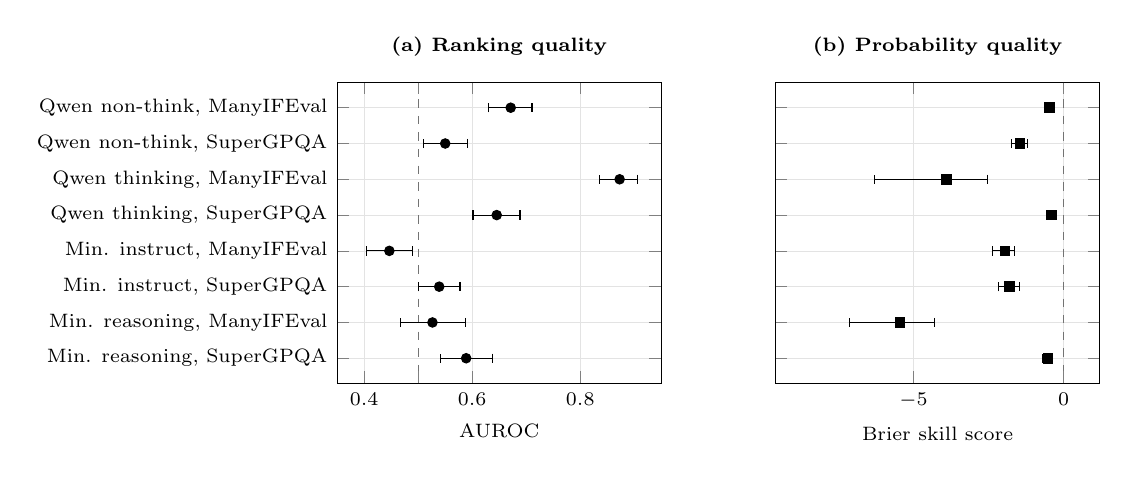
\begin{tikzpicture}
\pgfplotsset{
  cpisrow/.style={
    width=0.47\textwidth, height=5.4cm,
    ytick={0,1,2,3,4,5,6,7}, yticklabels={{Qwen non-think, ManyIFEval},{Qwen non-think, SuperGPQA},{Qwen thinking, ManyIFEval},{Qwen thinking, SuperGPQA},{Min. instruct, ManyIFEval},{Min. instruct, SuperGPQA},{Min. reasoning, ManyIFEval},{Min. reasoning, SuperGPQA}},
    y dir=reverse, ymin=-0.7, ymax=7.7,
    tick label style={font=\scriptsize}, label style={font=\scriptsize},
    title style={font=\scriptsize\bfseries},
    grid=major, grid style={gray!22,very thin},
  },
}
\begin{axis}[cpisrow, name=left, xlabel={AUROC}, title={(a) Ranking quality},
  xmin=0.35, xmax=0.95, extra x ticks={0.5}, extra x tick style={grid=major,
  grid style={black!55,dashed}, xticklabel=\empty}]
\addplot[only marks, mark=*, mark size=1.7pt, color=black,
  error bars/.cd, x dir=both, x explicit, error bar style={black}]
  coordinates {(0.6713,0) += (0.0395,0) -= (0.0409,0) (0.5501,1) += (0.0411,0) -= (0.0402,0) (0.8729,2) += (0.0325,0) -= (0.0376,0) (0.6454,3) += (0.0432,0) -= (0.0439,0) (0.4467,4) += (0.0427,0) -= (0.0426,0) (0.5390,5) += (0.0385,0) -= (0.0390,0) (0.5265,6) += (0.0610,0) -= (0.0594,0) (0.5889,7) += (0.0479,0) -= (0.0470,0)};
\end{axis}
\begin{axis}[cpisrow, at={(left.south east)}, xshift=1.45cm, anchor=south west,
  yticklabels=\empty, xlabel={Brier skill score}, title={(b) Probability quality},
  xmin=-9.6, xmax=1.2, extra x ticks={0}, extra x tick style={grid=major,
  grid style={black!55,dashed}, xticklabel=\empty}]
\addplot[only marks, mark=square*, mark size=1.7pt, color=black,
  error bars/.cd, x dir=both, x explicit, error bar style={black}]
  coordinates {(-0.4635,0) += (0.1127,0) -= (0.1272,0) (-1.4505,1) += (0.2322,0) -= (0.2756,0) (-3.8944,2) += (1.3576,0) -= (2.4000,0) (-0.4109,3) += (0.1117,0) -= (0.1174,0) (-1.9518,4) += (0.3235,0) -= (0.4105,0) (-1.7952,5) += (0.3135,0) -= (0.3803,0) (-5.4471,6) += (1.1453,0) -= (1.6982,0) (-0.5238,7) += (0.1478,0) -= (0.1699,0)};
\end{axis}
\end{tikzpicture}

\vspace{1.5ex}

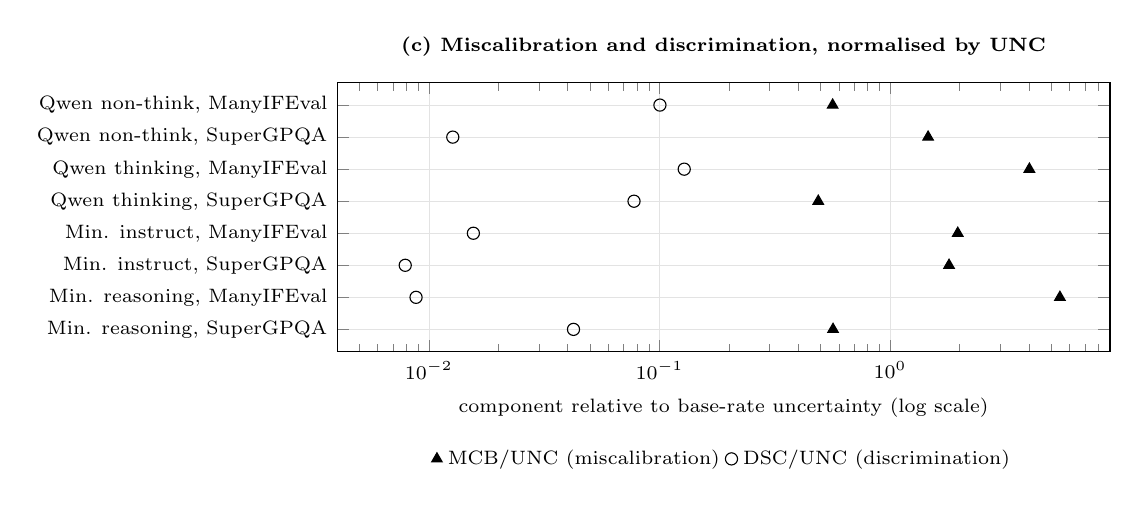
\begin{tikzpicture}
\begin{axis}[
  width=0.94\textwidth, height=5.0cm,
  ytick={0,1,2,3,4,5,6,7}, yticklabels={{Qwen non-think, ManyIFEval},{Qwen non-think, SuperGPQA},{Qwen thinking, ManyIFEval},{Qwen thinking, SuperGPQA},{Min. instruct, ManyIFEval},{Min. instruct, SuperGPQA},{Min. reasoning, ManyIFEval},{Min. reasoning, SuperGPQA}}, y dir=reverse,
  ymin=-0.7, ymax=7.7,
  xmode=log, xmin=0.004, xmax=9,
  xlabel={component relative to base-rate uncertainty (log scale)},
  title style={font=\scriptsize\bfseries},
  title={(c) Miscalibration and discrimination, normalised by UNC},
  tick label style={font=\scriptsize}, label style={font=\scriptsize},
  legend style={font=\scriptsize, at={(0.5,-0.32)}, anchor=north, legend columns=2, draw=none},
  grid=major, grid style={gray!22,very thin}]
\addplot[only marks, mark=triangle*, mark size=2.2pt, color=black] coordinates {(0.5640,0) (1.4631,1) (4.0225,2) (0.4885,3) (1.9675,4) (1.8031,5) (5.4559,6) (0.5662,7)};
\addlegendentry{MCB/UNC (miscalibration)}
\addplot[only marks, mark=o, mark size=2.2pt, color=black] coordinates {(0.1005,0) (0.0127,1) (0.1281,2) (0.0776,3) (0.0156,4) (0.0079,5) (0.0088,6) (0.0424,7)};
\addlegendentry{DSC/UNC (discrimination)}
\end{axis}
\end{tikzpicture}

\caption{Reference-configuration confidence quality, held-out data. (\textbf{a})
AUROC with 95\% item-bootstrap intervals; the dashed line is chance.
(\textbf{b}) Brier skill score against the base-rate forecast; the dashed line
is zero, and every interval lies below it. (\textbf{c}) Miscalibration (MCB) and
discrimination (DSC), each normalised by the base-rate uncertainty UNC, on a
logarithmic axis. Markers distinguish the quantities so the panel remains
readable without colour.\label{fig:refquality}}
\end{figure}

\subsection{Threshold viability and confidence quantisation}
\label{sec:thresholds}

Only \NumRiskTargetAttained{} of the \NumQualityPairs{} pairs admitted a threshold meeting
the \TargetRisk{} selective-risk target at any observed value; the remaining
\NumRiskTargetInfeasible{} fell back to the prespecified fixed-coverage target
(Table~\ref{tab:thresholds}). That a weak confidence signal fails to yield a
low-risk operating point is the scientifically correct outcome and the sample
was not enlarged to rescue it.

The fallback overshoots its nominal coverage, reaching \OvershootCoverage{} for
\OvershootModel{} on \OvershootDataset{} against a target of
\FixedCoverageTarget{}. This is structural rather than an optimisation failure.
Reported confidence is not continuous: models emit between
\MinDistinctConfidence{} and \MaxDistinctConfidence{} distinct values, and a
single atom can carry up to \MaxAtomMass{} of the mass. Coverage
$K(\tau)=P(C\ge\tau)$ is therefore a step function whose jumps are those atoms,
and a nominal coverage target below the largest atom's mass is simply not
reachable. Native verbal confidence does not support fine-grained threshold
control even where it carries usable ranking information.

\begin{table}[H]
\begin{adjustwidth}{-\extralength}{0cm}
\small
\caption{Frozen thresholds and the granularity of the confidence channel. The endpoint column records which branch of the prespecified rule applied. The last two columns describe the reported-confidence distribution at calibration.\label{tab:thresholds}}
\begin{tabular}{llllcccrl}
\toprule
\textbf{Model} & \textbf{Regime} & \textbf{Data} & \textbf{Endpoint} & $\boldsymbol{\tau_0}$ & \textbf{Coverage} & \textbf{Risk} & \textbf{Values} & \textbf{Top atom (mass)} \\
\midrule
Ministral-3-8B & instruct & ManyIFEval & coverage 0.50 & 0.98 & 0.637 & 0.670 & 9 & 0.98 (0.61) \tabularnewline
Ministral-3-8B & instruct & SuperGPQA & coverage 0.50 & 0.95 & 0.790 & 0.713 & 16 & 0.95 (0.73) \tabularnewline
Ministral-3-8B & reasoning & ManyIFEval & coverage 0.50 & 0.95 & 0.610 & 0.869 & 15 & 0.95 (0.44) \tabularnewline
Ministral-3-8B & reasoning & SuperGPQA & coverage 0.50 & 0.50 & 0.577 & 0.584 & 19 & 0.80 (0.13) \tabularnewline
Qwen3.5-9B & non-thinking & ManyIFEval & risk target & 1.00 & 0.230 & 0.087 & 12 & 0.95 (0.40) \tabularnewline
Qwen3.5-9B & non-thinking & SuperGPQA & coverage 0.50 & 1.00 & 0.627 & 0.665 & 11 & 1.00 (0.63) \tabularnewline
Qwen3.5-9B & thinking & ManyIFEval & coverage 0.50 & 0.10 & 0.650 & 0.892 & 21 & 0.00 (0.18) \tabularnewline
Qwen3.5-9B & thinking & SuperGPQA & coverage 0.50 & 0.95 & 0.693 & 0.370 & 17 & 0.95 (0.39) \tabularnewline
\bottomrule
\end{tabular}
\end{adjustwidth}
\end{table}


\subsection{Frozen-policy response to inference shift}
\label{sec:shift}

Table~\ref{tab:contrasts} and Figure~\ref{fig:forest} give the
\NumContrasts{} prespecified contrasts. After Holm correction,
\NumChangeDetected{} contrast shows a detected change in selective risk:
\DetectedModel{} on \DetectedDataset{} under the \DetectedShift{} shift, with
$\Delta R = \DetectedDeltaR$ $[\DetectedCILow, \DetectedCIHigh]$ and adjusted
$p = \DetectedHolmP$. \NumEquivalent{} contrast meets the equivalence criterion
and \NumInconclusive{} are inconclusive.

The single equivalence classification should not be read as a demonstration of
portability. In that contrast, neither the answer-change rate nor the
confidence-change rate exceeds \MaxRealisationEquivalent{}; in every other
contrast, at least one rate is \MinRealisationNonEquivalent{} or higher. The
equivalent contrast therefore also has the weakest manipulation check in the
panel. This does not show that the intervention had no effect.

The operational picture is different from the conditional one.
Table~\ref{tab:partition} and Figure~\ref{fig:endpoints} show the five outcomes.
\MaxCoverageModel{} on \MaxCoverageDataset{} under the \MaxCoverageShift{} shift
moves coverage by \MaxCoverageDeltaK{} while its selective risk moves only
\MaxCoverageDeltaR{}: the accepted-answer error rate changed little while the
policy stopped accepting more than a third of the work. Elsewhere answer
generation itself gives way, with \MaxAnswerFailModel{} on \MaxAnswerFailDataset{} showing
$\Delta q = \MaxAnswerFailDeltaQ{}$ under the \MaxAnswerFailShift{} shift. A
report restricted to $\Delta R$ would have described both as portable.

\begin{table}[H]
\begin{adjustwidth}{-\extralength}{0cm}
\footnotesize
\caption{The 16 prespecified held-out contrasts. $I_A$ and $I_C$ are the fractions of answer and confidence generations the shift changed. Intervals are 95\% item-clustered paired bootstrap; $p$ is Holm-adjusted within each model--dataset family.\label{tab:contrasts}}
\begin{tabular}{llllcccccccl}
\toprule
\textbf{Model} & \textbf{Regime} & \textbf{Data} & \textbf{Shift} & $\boldsymbol{I_A}$ & $\boldsymbol{I_C}$ & $\boldsymbol{\Delta q}$ & $\boldsymbol{\Delta K}$ & $\boldsymbol{\Delta R}$ \textbf{(95\% CI)} & $\boldsymbol{\Delta S}$ & \textbf{Holm} $\boldsymbol{p}$ & \textbf{Class} \\
\midrule
Ministral-3-8B & instruct & ManyIFEval & high-$T$ & 1.00 & 0.82 & +0.000 & -0.322 & -0.052 [-0.118, +0.010] & -0.067 & 0.876 & inconclusive \tabularnewline
Ministral-3-8B & instruct & ManyIFEval & low-$p$ & 0.71 & 0.21 & +0.000 & +0.017 & -0.030 [-0.056, -0.005] & +0.025 & 0.234 & inconclusive \tabularnewline
Ministral-3-8B & instruct & SuperGPQA & high-$T$ & 0.36 & 0.74 & +0.000 & -0.357 & +0.011 [-0.037, +0.059] & -0.120 & 1.000 & inconclusive \tabularnewline
Ministral-3-8B & instruct & SuperGPQA & low-$p$ & 0.01 & 0.01 & +0.000 & +0.003 & +0.003 [-0.004, +0.011] & -0.002 & 1.000 & equivalent \tabularnewline
Ministral-3-8B & reasoning & ManyIFEval & high-$T$ & 1.00 & 0.86 & +0.000 & -0.072 & +0.017 [-0.018, +0.051] & -0.018 & 1.000 & inconclusive \tabularnewline
Ministral-3-8B & reasoning & ManyIFEval & low-$p$ & 1.00 & 0.74 & +0.000 & +0.053 & +0.018 [-0.013, +0.050] & -0.005 & 1.000 & inconclusive \tabularnewline
Ministral-3-8B & reasoning & SuperGPQA & high-$T$ & 0.83 & 0.56 & -0.017 & +0.037 & +0.053 [+0.012, +0.095] & -0.017 & 0.171 & inconclusive \tabularnewline
Ministral-3-8B & reasoning & SuperGPQA & low-$p$ & 0.86 & 0.72 & +0.153 & -0.142 & +0.045 [-0.009, +0.102] & -0.087 & 1.000 & inconclusive \tabularnewline
Qwen3.5-9B & non-thinking & ManyIFEval & high-$T$ & 1.00 & 0.79 & +0.000 & +0.033 & +0.067 [-0.023, +0.156] & +0.007 & 1.000 & inconclusive \tabularnewline
Qwen3.5-9B & non-thinking & ManyIFEval & low-$p$ & 0.93 & 0.58 & +0.000 & -0.007 & -0.036 [-0.112, +0.044] & +0.003 & 1.000 & inconclusive \tabularnewline
Qwen3.5-9B & non-thinking & SuperGPQA & high-$T$ & 0.22 & 0.29 & +0.000 & -0.065 & +0.036 [+0.005, +0.067] & -0.047 & 0.302 & inconclusive \tabularnewline
Qwen3.5-9B & non-thinking & SuperGPQA & low-$p$ & 0.06 & 0.12 & +0.000 & +0.028 & -0.008 [-0.030, +0.015] & +0.017 & 1.000 & inconclusive \tabularnewline
Qwen3.5-9B & thinking & ManyIFEval & high-$T$ & 1.00 & 1.00 & +0.000 & +0.087 & +0.016 [+0.007, +0.026] & -0.003 & 0.003 & change \tabularnewline
Qwen3.5-9B & thinking & ManyIFEval & low-$p$ & 1.00 & 1.00 & +0.000 & -0.113 & -0.013 [-0.027, -0.001] & -0.003 & 0.306 & inconclusive \tabularnewline
Qwen3.5-9B & thinking & SuperGPQA & high-$T$ & 1.00 & 1.00 & +0.002 & -0.057 & -0.004 [-0.040, +0.033] & -0.033 & 1.000 & inconclusive \tabularnewline
Qwen3.5-9B & thinking & SuperGPQA & low-$p$ & 1.00 & 1.00 & +0.000 & +0.083 & -0.001 [-0.037, +0.034] & +0.053 & 1.000 & inconclusive \tabularnewline
\bottomrule
\end{tabular}
\end{adjustwidth}
\end{table}


\begin{figure}[H]
\centering

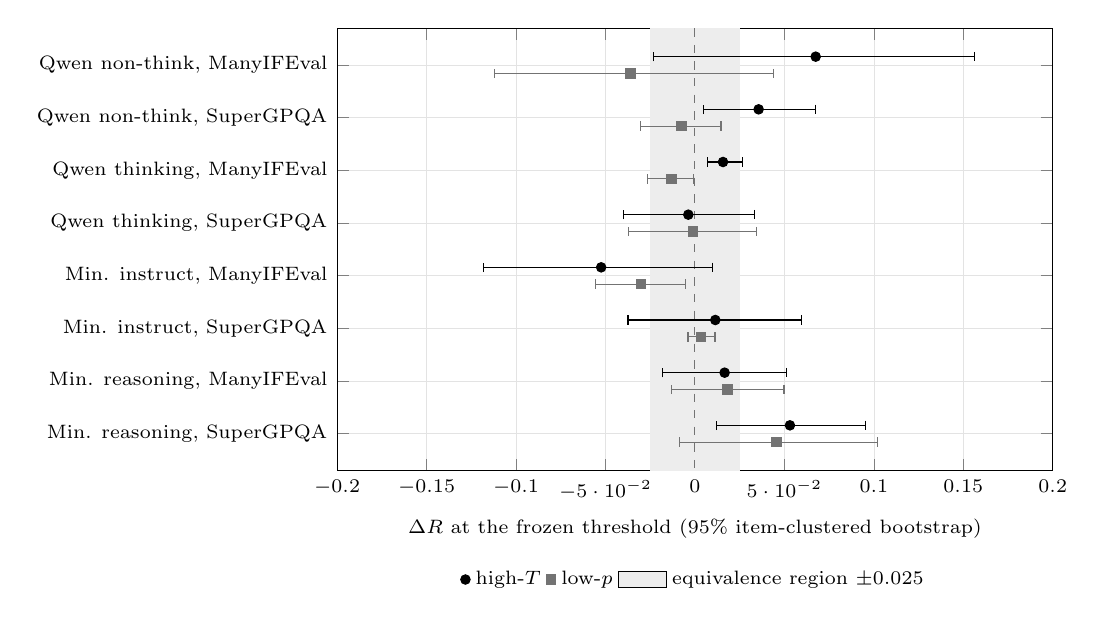
\begin{tikzpicture}
\begin{axis}[
  width=0.88\textwidth, height=7.2cm,
  ytick={0,1,2,3,4,5,6,7}, yticklabels={{Qwen non-think, ManyIFEval},{Qwen non-think, SuperGPQA},{Qwen thinking, ManyIFEval},{Qwen thinking, SuperGPQA},{Min. instruct, ManyIFEval},{Min. instruct, SuperGPQA},{Min. reasoning, ManyIFEval},{Min. reasoning, SuperGPQA}}, y dir=reverse,
  ymin=-0.7, ymax=7.7,
  xmin=-0.20, xmax=0.20,
  xlabel={$\Delta R$ at the frozen threshold (95\% item-clustered bootstrap)},
  tick label style={font=\scriptsize}, label style={font=\scriptsize},
  legend style={font=\scriptsize, at={(0.5,-0.20)}, anchor=north, legend columns=3, draw=none},
  grid=major, grid style={gray!22,very thin}]
\fill[black!7] (axis cs:-0.025,-0.7) rectangle (axis cs:0.025,7.7);
\draw[black!55,dashed] (axis cs:0,-0.7) -- (axis cs:0,7.7);
\addplot[only marks, mark=*, mark size=1.7pt, color=black,
  error bars/.cd, x dir=both, x explicit, error bar style={black}]
  coordinates {(0.0675,-0.16) += (0.0889,0) -= (0.0908,0) (0.0356,0.84) += (0.0318,0) -= (0.0308,0) (0.0157,1.84) += (0.0108,0) -= (0.0088,0) (-0.0037,2.84) += (0.0368,0) -= (0.0363,0) (-0.0524,3.84) += (0.0620,0) -= (0.0660,0) (0.0114,4.84) += (0.0480,0) -= (0.0488,0) (0.0166,5.84) += (0.0344,0) -= (0.0346,0) (0.0531,6.84) += (0.0424,0) -= (0.0411,0)};
\addlegendentry{high-$T$}
\addplot[only marks, mark=square*, mark size=1.7pt, color=black!55,
  error bars/.cd, x dir=both, x explicit, error bar style={black!55}]
  coordinates {(-0.0361,0.16) += (0.0799,0) -= (0.0757,0) (-0.0076,1.16) += (0.0222,0) -= (0.0228,0) (-0.0132,2.16) += (0.0123,0) -= (0.0133,0) (-0.0011,3.16) += (0.0356,0) -= (0.0359,0) (-0.0302,4.16) += (0.0248,0) -= (0.0256,0) (0.0035,5.16) += (0.0077,0) -= (0.0074,0) (0.0183,6.16) += (0.0315,0) -= (0.0315,0) (0.0455,7.16) += (0.0563,0) -= (0.0540,0)};
\addlegendentry{low-$p$}
\addlegendimage{area legend, fill=black!7, draw=none}
\addlegendentry{equivalence region $\pm0.025$}
\end{axis}
\end{tikzpicture}

\caption{Change in selective risk at the frozen threshold, one interval per
contrast. The shaded band is the prespecified equivalence region. Estimates are
never pooled across model conditions, datasets or shifts.\label{fig:forest}}
\end{figure}

\begin{table}[H]
\begin{adjustwidth}{-\extralength}{0cm}
\footnotesize
\caption{The outcome partition. $S$ and $E$ at the reference configuration, then the change in each of the five disjoint components under each shift. By construction $S+E+q+a_C+a_\tau=1$ and $K=S+E$.\label{tab:partition}}
\begin{tabular}{llllccccccc}
\toprule
\textbf{Model} & \textbf{Regime} & \textbf{Data} & \textbf{Shift} & $\boldsymbol{S_0}$ & $\boldsymbol{E_0}$ & $\boldsymbol{\Delta S}$ & $\boldsymbol{\Delta E}$ & $\boldsymbol{\Delta q}$ & $\boldsymbol{\Delta a_C}$ & $\boldsymbol{\Delta a_\tau}$ \\
\midrule
Ministral-3-8B & instruct & ManyIFEval & high-$T$ & 0.175 & 0.490 & -0.067 & -0.255 & +0.000 & +0.000 & +0.322 \tabularnewline
Ministral-3-8B & instruct & ManyIFEval & low-$p$ & 0.175 & 0.490 & +0.025 & -0.008 & +0.000 & +0.000 & -0.017 \tabularnewline
Ministral-3-8B & instruct & SuperGPQA & high-$T$ & 0.253 & 0.532 & -0.120 & -0.237 & +0.000 & +0.000 & +0.357 \tabularnewline
Ministral-3-8B & instruct & SuperGPQA & low-$p$ & 0.253 & 0.532 & -0.002 & +0.005 & +0.000 & +0.000 & -0.003 \tabularnewline
Ministral-3-8B & reasoning & ManyIFEval & high-$T$ & 0.080 & 0.525 & -0.018 & -0.053 & +0.000 & -0.007 & +0.078 \tabularnewline
Ministral-3-8B & reasoning & ManyIFEval & low-$p$ & 0.080 & 0.525 & -0.005 & +0.058 & +0.000 & +0.022 & -0.075 \tabularnewline
Ministral-3-8B & reasoning & SuperGPQA & high-$T$ & 0.278 & 0.320 & -0.017 & +0.053 & -0.017 & -0.037 & +0.017 \tabularnewline
Ministral-3-8B & reasoning & SuperGPQA & low-$p$ & 0.278 & 0.320 & -0.087 & -0.055 & +0.153 & +0.085 & -0.097 \tabularnewline
Qwen3.5-9B & non-thinking & ManyIFEval & high-$T$ & 0.177 & 0.060 & +0.007 & +0.027 & +0.000 & +0.000 & -0.033 \tabularnewline
Qwen3.5-9B & non-thinking & ManyIFEval & low-$p$ & 0.177 & 0.060 & +0.003 & -0.010 & +0.000 & +0.000 & +0.007 \tabularnewline
Qwen3.5-9B & non-thinking & SuperGPQA & high-$T$ & 0.257 & 0.362 & -0.047 & -0.018 & +0.000 & +0.000 & +0.065 \tabularnewline
Qwen3.5-9B & non-thinking & SuperGPQA & low-$p$ & 0.257 & 0.362 & +0.017 & +0.012 & +0.000 & +0.000 & -0.028 \tabularnewline
Qwen3.5-9B & thinking & ManyIFEval & high-$T$ & 0.053 & 0.557 & -0.003 & +0.090 & +0.000 & -0.005 & -0.082 \tabularnewline
Qwen3.5-9B & thinking & ManyIFEval & low-$p$ & 0.053 & 0.557 & -0.003 & -0.110 & +0.000 & +0.205 & -0.092 \tabularnewline
Qwen3.5-9B & thinking & SuperGPQA & high-$T$ & 0.433 & 0.255 & -0.033 & -0.023 & +0.002 & -0.002 & +0.057 \tabularnewline
Qwen3.5-9B & thinking & SuperGPQA & low-$p$ & 0.433 & 0.255 & +0.053 & +0.030 & +0.000 & +0.008 & -0.092 \tabularnewline
\bottomrule
\end{tabular}
\end{adjustwidth}
\end{table}


\begin{figure}[H]
\centering

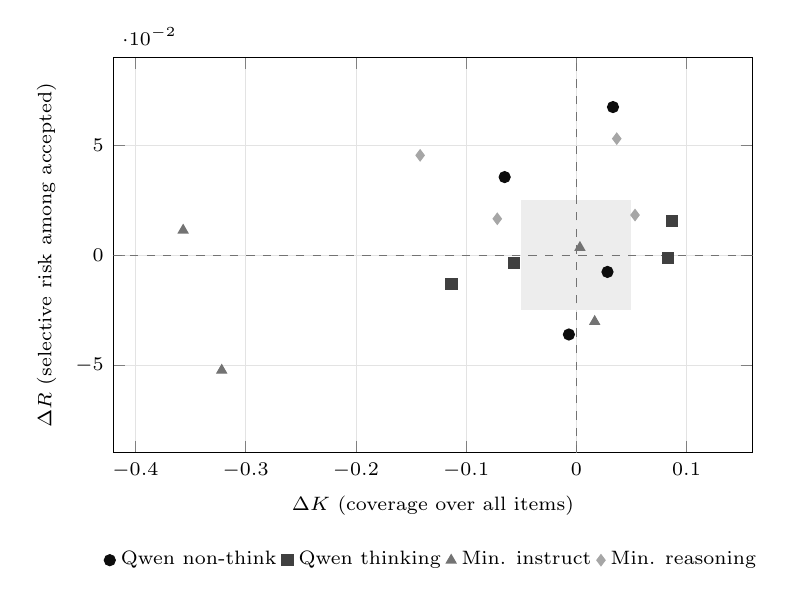
\begin{tikzpicture}
\begin{axis}[
  width=0.80\textwidth, height=6.6cm,
  xlabel={$\Delta K$ (coverage over all items)},
  ylabel={$\Delta R$ (selective risk among accepted)},
  xmin=-0.42, xmax=0.16, ymin=-0.09, ymax=0.09,
  tick label style={font=\scriptsize}, label style={font=\scriptsize},
  legend style={font=\scriptsize, at={(0.5,-0.22)}, anchor=north, legend columns=4, draw=none},
  grid=major, grid style={gray!22,very thin}]
\fill[black!7] (axis cs:-0.05,-0.025) rectangle (axis cs:0.05,0.025);
\draw[black!55,dashed] (axis cs:-0.42,0) -- (axis cs:0.16,0);
\draw[black!55,dashed] (axis cs:0,-0.09) -- (axis cs:0,0.09);
\addplot[only marks, mark=*, mark size=2.0pt, color=black!95] coordinates {(0.0333,0.0675) (-0.0067,-0.0361) (-0.0650,0.0356) (0.0283,-0.0076)};
\addlegendentry{Qwen non-think}
\addplot[only marks, mark=square*, mark size=2.0pt, color=black!75] coordinates {(0.0867,0.0157) (-0.1133,-0.0132) (-0.0567,-0.0037) (0.0833,-0.0011)};
\addlegendentry{Qwen thinking}
\addplot[only marks, mark=triangle*, mark size=2.0pt, color=black!55] coordinates {(-0.3217,-0.0524) (0.0167,-0.0302) (-0.3567,0.0114) (0.0033,0.0035)};
\addlegendentry{Min. instruct}
\addplot[only marks, mark=diamond*, mark size=2.0pt, color=black!35] coordinates {(-0.0717,0.0166) (0.0533,0.0183) (0.0367,0.0531) (-0.1417,0.0455)};
\addlegendentry{Min. reasoning}
\end{axis}
\end{tikzpicture}

\caption{Change in coverage against change in selective risk, one point per
contrast. The shaded rectangle is the joint equivalence region. Points far to
the left sit near $\Delta R = 0$ while the policy accepts far less work, which
is the case a conditional endpoint alone cannot
distinguish.\label{fig:endpoints}}
\end{figure}

\subsection{Precision of selective-risk estimates}
\label{sec:precision}

The predominance of inconclusive contrasts is largely a statement about
precision. Selective risk is estimated only on accepted items, so its relevant
denominator is the accepted count, approximately $NK$, rather than all $N$
items. Across the panel the accepted count ranges from \MinAcceptedN{} to
\MaxAcceptedN{} out of \NumHeldOutItems{} items.

Table~\ref{tab:precision} compares each 95\% interval against the width of
the equivalence region it would have to fit inside. For \NumCannotFitBand{} of
\NumContrasts{} contrasts the interval is wider than the whole region,
reaching \MaxWidthRatio{} times its width, so no equivalence classification was
available at the precision achieved, wherever the interval was centred. Only
\NumCanFitBand{} contrasts had sufficient precision, and \NumEquivalent{} of
those fell inside.

This describes the precision achieved here rather than a fixed limit of the design: a
different true risk at the same $N$ would produce a different width. What it
does expose is that an equivalence margin fixed without reference to coverage
can be unreachable for a pair that accepts few items.

\begin{table}[H]
\begin{adjustwidth}{-\extralength}{0cm}
\small
\caption{Precision of the selective-risk contrasts against the equivalence region. The accepted count is $NK$ at the reference configuration. The last column records whether the 95\% interval could have fitted inside the region at all.\label{tab:precision}}
\begin{tabular}{llllcrccl}
\toprule
\textbf{Model} & \textbf{Regime} & \textbf{Data} & \textbf{Shift} & \textbf{Accepted} $\boldsymbol{n}$ & \textbf{SE} & \textbf{CI width} & \textbf{vs band} & \textbf{Could fit} \\
\midrule
Ministral-3-8B & instruct & ManyIFEval & high-$T$ & 382 & 0.024 & 0.128 & 2.6$\times$ & \textbf{no} \tabularnewline
Ministral-3-8B & instruct & ManyIFEval & low-$p$ & 382 & 0.024 & 0.050 & 1.0$\times$ & \textbf{no} \tabularnewline
Ministral-3-8B & instruct & SuperGPQA & high-$T$ & 474 & 0.021 & 0.097 & 1.9$\times$ & \textbf{no} \tabularnewline
Ministral-3-8B & instruct & SuperGPQA & low-$p$ & 474 & 0.021 & 0.015 & 0.3$\times$ & yes \tabularnewline
Ministral-3-8B & reasoning & ManyIFEval & high-$T$ & 366 & 0.018 & 0.069 & 1.4$\times$ & \textbf{no} \tabularnewline
Ministral-3-8B & reasoning & ManyIFEval & low-$p$ & 366 & 0.018 & 0.063 & 1.3$\times$ & \textbf{no} \tabularnewline
Ministral-3-8B & reasoning & SuperGPQA & high-$T$ & 346 & 0.026 & 0.083 & 1.7$\times$ & \textbf{no} \tabularnewline
Ministral-3-8B & reasoning & SuperGPQA & low-$p$ & 346 & 0.026 & 0.110 & 2.2$\times$ & \textbf{no} \tabularnewline
Qwen3.5-9B & non-thinking & ManyIFEval & high-$T$ & 138 & 0.024 & 0.180 & 3.6$\times$ & \textbf{no} \tabularnewline
Qwen3.5-9B & non-thinking & ManyIFEval & low-$p$ & 138 & 0.024 & 0.156 & 3.1$\times$ & \textbf{no} \tabularnewline
Qwen3.5-9B & non-thinking & SuperGPQA & high-$T$ & 376 & 0.024 & 0.063 & 1.3$\times$ & \textbf{no} \tabularnewline
Qwen3.5-9B & non-thinking & SuperGPQA & low-$p$ & 376 & 0.024 & 0.045 & 0.9$\times$ & yes \tabularnewline
Qwen3.5-9B & thinking & ManyIFEval & high-$T$ & 390 & 0.016 & 0.020 & 0.4$\times$ & yes \tabularnewline
Qwen3.5-9B & thinking & ManyIFEval & low-$p$ & 390 & 0.016 & 0.026 & 0.5$\times$ & yes \tabularnewline
Qwen3.5-9B & thinking & SuperGPQA & high-$T$ & 416 & 0.024 & 0.073 & 1.5$\times$ & \textbf{no} \tabularnewline
Qwen3.5-9B & thinking & SuperGPQA & low-$p$ & 416 & 0.024 & 0.072 & 1.4$\times$ & \textbf{no} \tabularnewline
\bottomrule
\end{tabular}
\end{adjustwidth}
\end{table}


\subsection{Observed output changes across model regimes}
\label{sec:realisation}

The same nominal decoder change is not a common treatment.
Figure~\ref{fig:realisation} plots $I_A$ against $I_C$ for every contrast.
The observed change rates span nearly the full range: at one extreme a shift
changes every answer and every confidence, while at the other it changes almost
nothing. Anchoring
each shift on the model's native configuration is what produces this, and it is
the honest way to shift a decoder, but it means an experiment comparing
``temperature effects'' across models is not comparing equal interventions.

The two outputs also move differently. Points off the diagonal in
Figure~\ref{fig:realisation} are contrasts where the confidence output changed
far more, or far less, often than the answer output. Restricting to items whose
answers came back byte-identical isolates readout-side movement on that subset;
where that subset exists, the conditional rates differ sharply across contrasts.
\NumAllAnswersChanged{} of the \NumContrasts{} contrasts changed every compared answer and leave
no such subset, and are reported as undefined rather than as zero. We do not
describe this as mediation: a mediation claim would require the crossed
counterfactuals in which the readout at one configuration is applied to the answer
produced at another, and those cells were deliberately not generated. The
defensible statement is that verifying an inference intervention by inspecting
final answers alone can understate how strongly it perturbed a confidence-based
system.

\begin{figure}[H]
\centering

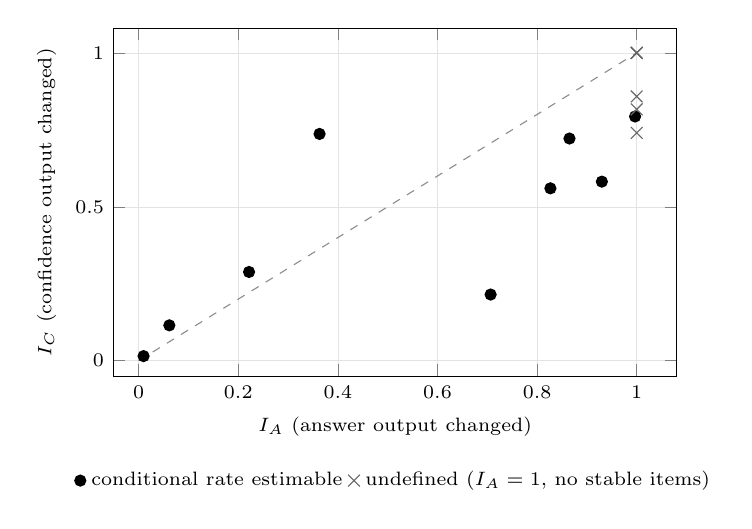
\begin{tikzpicture}
\begin{axis}[
  width=0.72\textwidth, height=6.0cm,
  xlabel={$I_A$ (answer output changed)},
  ylabel={$I_C$ (confidence output changed)},
  xmin=-0.05, xmax=1.08, ymin=-0.05, ymax=1.08,
  tick label style={font=\scriptsize}, label style={font=\scriptsize},
  legend style={font=\scriptsize, at={(0.5,-0.24)}, anchor=north, legend columns=2, draw=none},
  grid=major, grid style={gray!22,very thin}]
\addplot[domain=0:1, samples=2, black!45, dashed, forget plot] {x};
\addplot[only marks, mark=*, mark size=2.0pt, color=black] coordinates {(0.9967,0.7933) (0.9300,0.5817) (0.2217,0.2883) (0.0617,0.1150) (0.7067,0.2150) (0.3633,0.7367) (0.0100,0.0150) (0.8267,0.5600) (0.8650,0.7217)};
\addlegendentry{conditional rate estimable}
\addplot[only marks, mark=x, mark size=3.0pt, color=black!60] coordinates {(1.0000,1.0000) (1.0000,1.0000) (1.0000,1.0000) (1.0000,1.0000) (1.0000,0.8167) (1.0000,0.8583) (1.0000,0.7400)};
\addlegendentry{undefined ($I_A=1$, no stable items)}
\end{axis}
\end{tikzpicture}

\caption{Observed output changes per contrast. $I_A$ is the fraction of answer
generations the shift changed and $I_C$ the fraction of confidence generations.
The dashed diagonal marks equal change rates in the two outputs. Crosses mark
contrasts that changed every answer, for which the conditional rate is
undefined rather than zero.\label{fig:realisation}}
\end{figure}

\subsection{Sensitivity to sampling seed}
\label{sec:seeds}

The broad study runs one sampling seed. A secondary subset of
\SeedSubsetItems{} items per dataset, drawn from inside the held-out window,
repeats all conditions at \NumSeeds{} seeds (\SeedList{}) at the same frozen
thresholds. All \NumSeeds{} seeds were regenerated in this run rather than
reusing the broad study's records, because generation on this engine is not
invariant to batch composition and reuse would have confounded the seed contrast
with a change of batching. What is measured is therefore the variability of a
rerun under one batching regime.

The direction of the effect is often not stable. Of \NumSeedContrasts{} risk
contrasts, \NumSeedSignFlipRisk{} change sign across the \NumSeeds{} seeds, and
\NumSeedSignFlipAll{} of \NumSeedEndpointCombos{} contrast--endpoint
combinations do (Figure~\ref{fig:seeds}, Table~\ref{tab:seeds}). For
\NumSeedSDExceedsMargin{} contrasts the across-seed standard deviation alone,
reaching \MaxSeedSD{}, exceeds the entire equivalence half-margin of
\MarginRisk{}.

The variance split of Equation~\eqref{eq:lotv} is consistent with this. Across
the \NumVarianceSplits{} contrast--endpoint combinations that admit a split, the
share attributable to resampling the decoder exceeds one half in
\NumSeedShareAboveHalf{} of them, with median \MedianSeedShare{} and a range
from \MinSeedShare{} to \MaxSeedShare{}. This is a description of this panel and
not a property of every contrast, and \NumSeeds{} seeds on
\SeedSubsetItems{} items cannot characterise a distribution over seeds.
The consequence for the primary analysis is nonetheless clear: the
item-clustered intervals of Section~\ref{sec:shift} are intervals around
$\Delta_{s_0}$, and they can materially understate variability across
sampling runs.

\begin{figure}[H]
\centering

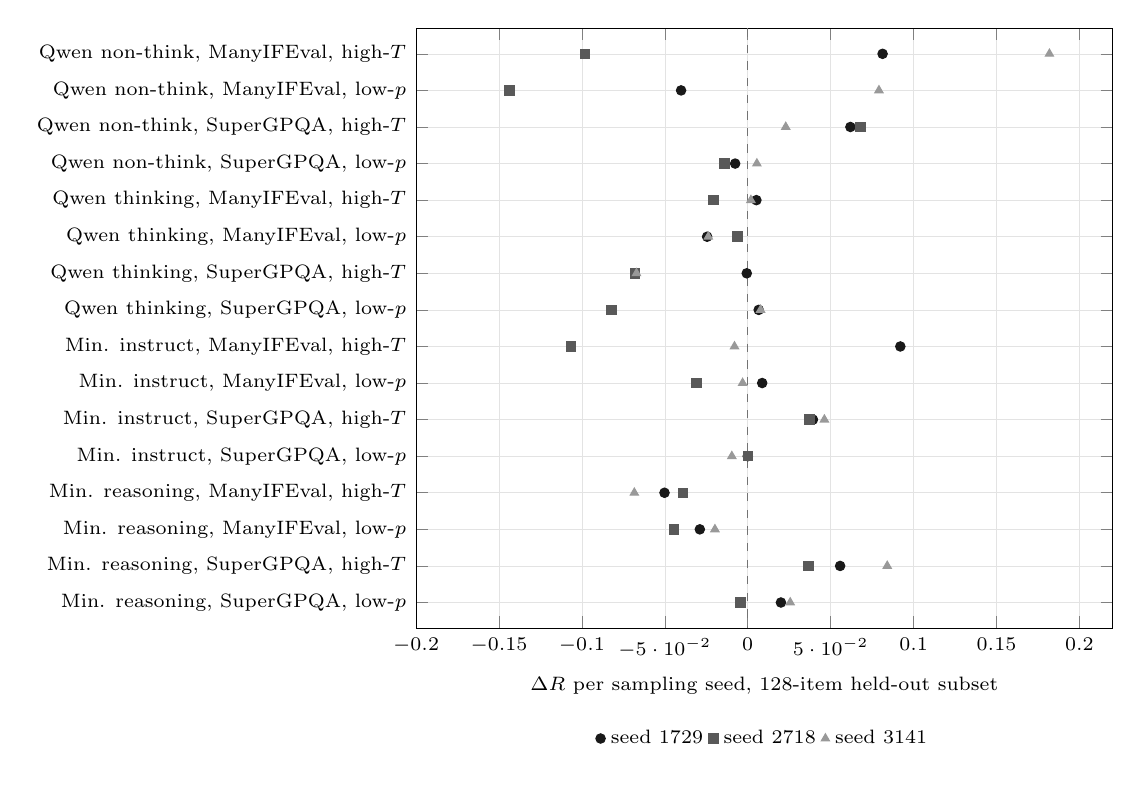
\begin{tikzpicture}
\begin{axis}[
  width=0.86\textwidth, height=9.2cm,
  ytick={0,1,2,3,4,5,6,7,8,9,10,11,12,13,14,15}, yticklabels={{Qwen non-think, ManyIFEval, high-$T$},{Qwen non-think, ManyIFEval, low-$p$},{Qwen non-think, SuperGPQA, high-$T$},{Qwen non-think, SuperGPQA, low-$p$},{Qwen thinking, ManyIFEval, high-$T$},{Qwen thinking, ManyIFEval, low-$p$},{Qwen thinking, SuperGPQA, high-$T$},{Qwen thinking, SuperGPQA, low-$p$},{Min. instruct, ManyIFEval, high-$T$},{Min. instruct, ManyIFEval, low-$p$},{Min. instruct, SuperGPQA, high-$T$},{Min. instruct, SuperGPQA, low-$p$},{Min. reasoning, ManyIFEval, high-$T$},{Min. reasoning, ManyIFEval, low-$p$},{Min. reasoning, SuperGPQA, high-$T$},{Min. reasoning, SuperGPQA, low-$p$}}, y dir=reverse,
  ymin=-0.7, ymax=15.7,
  xmin=-0.20, xmax=0.22,
  xlabel={$\Delta R$ per sampling seed, 128-item held-out subset},
  tick label style={font=\scriptsize}, label style={font=\scriptsize},
  legend style={font=\scriptsize, at={(0.5,-0.15)}, anchor=north, legend columns=3, draw=none},
  grid=major, grid style={gray!22,very thin}]
\draw[black!55,dashed] (axis cs:0,-0.7) -- (axis cs:0,15.7);
\addplot[only marks, mark=*, mark size=1.7pt, color=black!90] coordinates {(0.0813,0) (-0.0402,1) (0.0619,2) (-0.0076,3) (0.0052,4) (-0.0245,5) (-0.0006,6) (0.0066,7) (0.0920,8) (0.0087,9) (0.0393,10) (0.0000,11) (-0.0502,12) (-0.0289,13) (0.0557,14) (0.0200,15)};
\addlegendentry{seed 1729}
\addplot[only marks, mark=square*, mark size=1.7pt, color=black!65] coordinates {(-0.0982,0) (-0.1437,1) (0.0679,2) (-0.0139,3) (-0.0206,4) (-0.0063,5) (-0.0679,6) (-0.0821,7) (-0.1067,8) (-0.0310,9) (0.0371,10) (0.0000,11) (-0.0390,12) (-0.0446,13) (0.0366,14) (-0.0044,15)};
\addlegendentry{seed 2718}
\addplot[only marks, mark=triangle*, mark size=1.7pt, color=black!40] coordinates {(0.1819,0) (0.0791,1) (0.0229,2) (0.0055,3) (0.0019,4) (-0.0238,5) (-0.0671,6) (0.0077,7) (-0.0080,8) (-0.0031,9) (0.0462,10) (-0.0096,11) (-0.0684,12) (-0.0198,13) (0.0841,14) (0.0256,15)};
\addlegendentry{seed 3141}
\end{axis}
\end{tikzpicture}

\caption{Change in selective risk at each of \NumSeeds{} sampling seeds on the
\SeedSubsetItems{}-item held-out subset. Rows whose markers fall on both sides
of zero are contrasts whose direction is not stable across sampling runs. This
is a secondary robustness subset and does not revise any
held-out classification.\label{fig:seeds}}
\end{figure}

\begin{table}[H]
\begin{adjustwidth}{-\extralength}{0cm}
\footnotesize
\caption{Seed robustness on the 128-item held-out subset. The variance share is the fraction of per-item contrast variability attributable to resampling the decoder; selective risk is a ratio with no per-item value and carries no split.\label{tab:seeds}}
\begin{tabular}{llllclccr}
\toprule
\textbf{Model} & \textbf{Regime} & \textbf{Data} & \textbf{Shift} & \textbf{Endpoint} & \textbf{Per-seed values} & \textbf{SD} & \textbf{Sign stable} & \textbf{Seed share} \\
\midrule
Ministral-3-8B & instruct & ManyIFEval & high-$T$ & $\Delta R$ & +0.092, -0.107, -0.008 & 0.081 & \textbf{no} & -- \tabularnewline
Ministral-3-8B & instruct & ManyIFEval & high-$T$ & $\Delta K$ & -0.383, -0.156, -0.297 & 0.093 & yes & 0.56 \tabularnewline
Ministral-3-8B & instruct & ManyIFEval & high-$T$ & $\Delta S$ & -0.148, +0.000, -0.109 & 0.063 & yes & 0.39 \tabularnewline
Ministral-3-8B & instruct & ManyIFEval & low-$p$ & $\Delta R$ & +0.009, -0.031, -0.003 & 0.017 & \textbf{no} & -- \tabularnewline
Ministral-3-8B & instruct & ManyIFEval & low-$p$ & $\Delta K$ & -0.008, -0.008, +0.016 & 0.011 & \textbf{no} & 0.62 \tabularnewline
Ministral-3-8B & instruct & ManyIFEval & low-$p$ & $\Delta S$ & -0.008, +0.016, +0.008 & 0.010 & \textbf{no} & 0.66 \tabularnewline
Ministral-3-8B & instruct & SuperGPQA & high-$T$ & $\Delta R$ & +0.039, +0.037, +0.046 & 0.004 & yes & -- \tabularnewline
Ministral-3-8B & instruct & SuperGPQA & high-$T$ & $\Delta K$ & -0.383, -0.375, -0.367 & 0.006 & yes & 0.46 \tabularnewline
Ministral-3-8B & instruct & SuperGPQA & high-$T$ & $\Delta S$ & -0.148, -0.141, -0.141 & 0.004 & yes & 0.54 \tabularnewline
Ministral-3-8B & instruct & SuperGPQA & low-$p$ & $\Delta R$ & +0.000, +0.000, -0.010 & 0.005 & yes & -- \tabularnewline
Ministral-3-8B & instruct & SuperGPQA & low-$p$ & $\Delta K$ & +0.000, +0.000, +0.000 & 0.000 & yes & -- \tabularnewline
Ministral-3-8B & instruct & SuperGPQA & low-$p$ & $\Delta S$ & +0.000, +0.000, +0.008 & 0.004 & yes & 0.67 \tabularnewline
Ministral-3-8B & reasoning & ManyIFEval & high-$T$ & $\Delta R$ & -0.050, -0.039, -0.068 & 0.012 & yes & -- \tabularnewline
Ministral-3-8B & reasoning & ManyIFEval & high-$T$ & $\Delta K$ & -0.078, -0.055, +0.047 & 0.054 & \textbf{no} & 0.71 \tabularnewline
Ministral-3-8B & reasoning & ManyIFEval & high-$T$ & $\Delta S$ & +0.016, +0.016, +0.047 & 0.015 & yes & 0.53 \tabularnewline
Ministral-3-8B & reasoning & ManyIFEval & low-$p$ & $\Delta R$ & -0.029, -0.045, -0.020 & 0.010 & yes & -- \tabularnewline
Ministral-3-8B & reasoning & ManyIFEval & low-$p$ & $\Delta K$ & +0.039, +0.094, +0.094 & 0.026 & yes & 0.64 \tabularnewline
Ministral-3-8B & reasoning & ManyIFEval & low-$p$ & $\Delta S$ & +0.023, +0.039, +0.023 & 0.007 & yes & 0.17 \tabularnewline
Ministral-3-8B & reasoning & SuperGPQA & high-$T$ & $\Delta R$ & +0.056, +0.037, +0.084 & 0.020 & yes & -- \tabularnewline
Ministral-3-8B & reasoning & SuperGPQA & high-$T$ & $\Delta K$ & +0.070, +0.000, -0.008 & 0.035 & \textbf{no} & 0.67 \tabularnewline
Ministral-3-8B & reasoning & SuperGPQA & high-$T$ & $\Delta S$ & +0.000, -0.023, -0.055 & 0.022 & yes & 0.50 \tabularnewline
Ministral-3-8B & reasoning & SuperGPQA & low-$p$ & $\Delta R$ & +0.020, -0.004, +0.026 & 0.013 & \textbf{no} & -- \tabularnewline
Ministral-3-8B & reasoning & SuperGPQA & low-$p$ & $\Delta K$ & -0.086, -0.055, -0.094 & 0.017 & yes & 0.59 \tabularnewline
Ministral-3-8B & reasoning & SuperGPQA & low-$p$ & $\Delta S$ & -0.055, -0.023, -0.062 & 0.017 & yes & 0.68 \tabularnewline
Qwen3.5-9B & non-thinking & ManyIFEval & high-$T$ & $\Delta R$ & +0.081, -0.098, +0.182 & 0.116 & \textbf{no} & -- \tabularnewline
Qwen3.5-9B & non-thinking & ManyIFEval & high-$T$ & $\Delta K$ & -0.016, +0.031, +0.086 & 0.042 & \textbf{no} & 0.67 \tabularnewline
Qwen3.5-9B & non-thinking & ManyIFEval & high-$T$ & $\Delta S$ & -0.031, +0.047, +0.023 & 0.033 & \textbf{no} & 0.59 \tabularnewline
Qwen3.5-9B & non-thinking & ManyIFEval & low-$p$ & $\Delta R$ & -0.040, -0.144, +0.079 & 0.091 & \textbf{no} & -- \tabularnewline
Qwen3.5-9B & non-thinking & ManyIFEval & low-$p$ & $\Delta K$ & -0.031, +0.008, +0.078 & 0.045 & \textbf{no} & 0.69 \tabularnewline
Qwen3.5-9B & non-thinking & ManyIFEval & low-$p$ & $\Delta S$ & -0.016, +0.039, +0.047 & 0.028 & \textbf{no} & -- \tabularnewline
Qwen3.5-9B & non-thinking & SuperGPQA & high-$T$ & $\Delta R$ & +0.062, +0.068, +0.023 & 0.020 & yes & -- \tabularnewline
Qwen3.5-9B & non-thinking & SuperGPQA & high-$T$ & $\Delta K$ & -0.086, -0.070, -0.023 & 0.027 & yes & 0.58 \tabularnewline
Qwen3.5-9B & non-thinking & SuperGPQA & high-$T$ & $\Delta S$ & -0.062, -0.062, -0.023 & 0.018 & yes & 0.58 \tabularnewline
Qwen3.5-9B & non-thinking & SuperGPQA & low-$p$ & $\Delta R$ & -0.008, -0.014, +0.006 & 0.008 & \textbf{no} & -- \tabularnewline
Qwen3.5-9B & non-thinking & SuperGPQA & low-$p$ & $\Delta K$ & +0.055, +0.062, +0.047 & 0.006 & yes & 0.55 \tabularnewline
Qwen3.5-9B & non-thinking & SuperGPQA & low-$p$ & $\Delta S$ & +0.023, +0.031, +0.016 & 0.006 & yes & 0.53 \tabularnewline
Qwen3.5-9B & thinking & ManyIFEval & high-$T$ & $\Delta R$ & +0.005, -0.021, +0.002 & 0.011 & \textbf{no} & -- \tabularnewline
Qwen3.5-9B & thinking & ManyIFEval & high-$T$ & $\Delta K$ & +0.039, -0.141, +0.016 & 0.080 & \textbf{no} & 0.62 \tabularnewline
Qwen3.5-9B & thinking & ManyIFEval & high-$T$ & $\Delta S$ & +0.000, -0.000, +0.000 & 0.000 & yes & -- \tabularnewline
Qwen3.5-9B & thinking & ManyIFEval & low-$p$ & $\Delta R$ & -0.025, -0.006, -0.024 & 0.008 & yes & -- \tabularnewline
Qwen3.5-9B & thinking & ManyIFEval & low-$p$ & $\Delta K$ & -0.203, -0.219, -0.148 & 0.030 & yes & 0.66 \tabularnewline
Qwen3.5-9B & thinking & ManyIFEval & low-$p$ & $\Delta S$ & -0.008, -0.016, -0.000 & 0.006 & yes & -- \tabularnewline
Qwen3.5-9B & thinking & SuperGPQA & high-$T$ & $\Delta R$ & -0.001, -0.068, -0.067 & 0.032 & yes & -- \tabularnewline
Qwen3.5-9B & thinking & SuperGPQA & high-$T$ & $\Delta K$ & -0.062, -0.055, -0.055 & 0.004 & yes & 0.62 \tabularnewline
Qwen3.5-9B & thinking & SuperGPQA & high-$T$ & $\Delta S$ & -0.039, +0.016, +0.016 & 0.026 & \textbf{no} & 0.78 \tabularnewline
Qwen3.5-9B & thinking & SuperGPQA & low-$p$ & $\Delta R$ & +0.007, -0.082, +0.008 & 0.042 & \textbf{no} & -- \tabularnewline
Qwen3.5-9B & thinking & SuperGPQA & low-$p$ & $\Delta K$ & +0.008, +0.062, +0.023 & 0.023 & yes & 0.68 \tabularnewline
Qwen3.5-9B & thinking & SuperGPQA & low-$p$ & $\Delta S$ & +0.000, +0.102, +0.008 & 0.046 & yes & 0.50 \tabularnewline
\bottomrule
\end{tabular}
\end{adjustwidth}
\end{table}


\section{Discussion}

\paragraph{Calibration, discrimination and decision utility are three
properties, not one.}
The panel separates them empirically. A confidence signal can order errors well
and still be unusable as a probability, as the \RankingCaseModel{} case shows,
and a threshold built on a well-ranked but badly scaled signal can still
deliver a workable operating point because thresholding uses only the ordering.
Conversely, a well-calibrated signal with no discrimination supports no useful
threshold at all. Reporting a single calibration number collapses distinctions
that matter operationally.

\paragraph{Conditional risk does not describe the whole system.}
The clearest practical lesson is that a fixed-threshold policy can keep nearly
the same selective risk and simultaneously stop doing its job. Because
$R = E/(S+E)$ and $K = S+E$, two configurations can agree on $R$ and disagree enormously on how
much autonomous work they deliver. Any monitoring scheme that watches only the
accepted-error rate will be blind to exactly the failure our largest coverage
movement exhibits.

\paragraph{Inference parameters are model-dependent interventions.}
A nominal temperature or top-$p$ change applied to two models is not the same
intervention, because each model's native configuration differs and because the
answer and confidence outputs respond differently. Studies that compare
``decoder effects'' across models should report how often each output changes;
inspecting final answers alone can understate the effect on the confidence pass.

\paragraph{More items do not substitute for repeated inference.}
This is the methodological point with the widest reach. A benchmark of several
hundred items can produce narrow item-bootstrap intervals. If every item was
generated once, those intervals average over items while conditioning on a
single sampling seed. Our seed subset shows that seed variation is frequently
the larger component. Enlarging the benchmark cannot help,
because it reduces a different variance component.

\paragraph{Consequences for deployment.}
Taken together, these results argue that a confidence threshold should be
treated as a property of a configuration rather than of a model. A policy
validated at one inference configuration should not be assumed valid at
another. Portability should be checked with a paired evaluation at the target
configuration that measures coverage and the full outcome partition as well as
selective risk.

\section{Limitations}

The design is deliberately narrow and the conclusions should not be read past
it. We study \NumModelFamilies{} open-weight model families in
\NumModelsConditions{} conditions and \NumDatasets{} benchmarks; nothing here
establishes behaviour for other families, for larger models, for proprietary
systems, or for tasks with different success events. We vary
\NumCoordinates{} inference configurations, one temperature increase and one nucleus
reduction per model, and make no claim about the full response surface or about
sampling algorithms we did not run.

The primary experiment uses a single sampling seed, and the repeated-seed study
covers \NumSeeds{} seeds on a \SeedSubsetItems{}-item subset, which is enough to
demonstrate that stochastic variability is material and not enough to
characterise its distribution. The seed subset is secondary and does not revise
any confirmatory classification.

Confidence is elicited by one coupled two-pass protocol; other elicitation
formats, standardized readouts and self-consistency procedures are outside this
design. The conditional confidence-change analysis is restricted to items whose
answers happened to be identical, a subset enriched for items the model answers
stably, and supports no causal mediation claim because the crossed readout cells
were not generated. Finally, the equivalence margins were fixed in advance
without reference to the coverage each pair would achieve, which
Section~\ref{sec:precision} shows left many contrasts unable to reach an
equivalence verdict.

\section{Conclusions}

We asked whether a confidence-based decision policy established under one
inference configuration remains statistically reliable when decoding settings
change, and we answer it as a characterisation rather than a verdict. At the
reference configuration, reported confidence is a poor probability forecast in
every pair we measured, while its ranking ability varies from unresolved to
strong. Probability quality and ranking ability are therefore distinct. Under
decoder shift, selective risk shows a Holm-adjusted change in
\NumChangeDetected{} of \NumContrasts{} contrasts,
but coverage, generation validity and operational success move substantially in
several, so a stable conditional risk does not imply a stable system. Much of
the remaining indeterminacy is a precision limit rather than evidence of
stability: a selective-risk estimate uses only the accepted items, and for
\NumCannotFitBand{} of \NumContrasts{} contrasts no equivalence
verdict was reachable. Finally, the same nominal decoder change does not produce
comparable output changes across models, and the measured effect frequently
depends more on the sampling seed than on which items were sampled.

The practical implication is that a confidence threshold is specific to the
configuration in which it was selected. Validation should use the intended
inference configuration and account for variation across sampling seeds;
monitoring should track coverage and the full outcome partition rather than the
accepted-answer error rate alone.

\vspace{6pt}

\supplementary{The analysis code, configuration files, frozen result artifacts
and the scripts that regenerate every table and figure in this article are
available in the repository named under Data Availability.}

\authorcontributions{Conceptualization, N.K., M.M., A.M.T. and S.K.;
methodology, N.K., A.M.T. and S.K.; software, N.K.; validation, N.K. and M.M.;
formal analysis, N.K.; investigation, N.K.; data curation, N.K.;
writing---original draft preparation, N.K.; writing---review and editing, N.K.,
M.M., A.M.T. and S.K.; visualization, N.K., A.M.T. and S.K.; supervision, M.M.;
project administration, N.K. and M.M. All authors have read and agreed to the
published version of the manuscript.}

\funding{Funding information to be confirmed by the authors prior to
submission.}

\institutionalreview{Not applicable.}

\informedconsent{Not applicable.}

\dataavailability{This study analyses existing public benchmarks and creates no
new human-subject data. The benchmarks used are SuperGPQA and ManyIFEval,
obtained from their public repositories at the exact revisions recorded in the
released configuration files, together with the checksums of the prepared
partition files, so that the evaluated item subsets can be reconstructed
deterministically. The benchmark corpora themselves are redistributed by their
original providers under their own licences and are not re-hosted here. The
model weights are the published open-weight releases identified by repository
and revision in the configuration files and are likewise not re-hosted. All
generated result artifacts required to reproduce every number, table and figure
in this article, together with the analysis code, are released in the
reproducibility repository; its URL is to be inserted on acceptance.}

\conflictsofinterest{To be confirmed by all authors prior to submission.}

\abbreviations{Abbreviations}{%
The following abbreviations are used in this manuscript:\\

\noindent
\begin{tabular}{@{}ll}
AUROC & Area under the receiver operating characteristic curve\\
BSS & Brier skill score\\
CORP & Consistent, optimally binned, reproducible, PAV-algorithm based\\
DSC & Discrimination component of the Brier score\\
LLM & Large language model\\
MCB & Miscalibration component of the Brier score\\
PAV & Pool-adjacent-violators\\
UNC & Uncertainty component of the Brier score
\end{tabular}
}

\begin{adjustwidth}{-\extralength}{0cm}
\reftitle{References}
\bibliography{cpis}
\end{adjustwidth}

\PublishersNote{}
\end{document}
